\section{Introduction}

    The application of exogenous-cross-links (EXLs) to native or biologically derived soft collagenous tissues finds its way into a wide range of medical therapies and device applications, such as surgical biomaterials, modification of corneal tissues (using riboflavin/UVA) and vascular grafts. Perhaps the most mechanically demanding application is the so-called bioprosthetic heart valve (BHV), which is fabricated from several types of biologically derived soft collagenous tissue membranes. From a clinical perspective, BHVs have important advantages in that they do not require permanent anticoagulation therapy, operate noiselessly, and have blood flow characteristics similar to the native valve, and thus have become the dominant heart valve therapy worldwide \cite{bini_noncollagenous_1999,schoen_cardiac_2005,schoen_founders_1999}. However, BHV durability continues to remain limited to the range of 10–15 years, resulting from leaflet structural deterioration mediated by fatigue and/or tissue mineralization \cite{vesely_tissue_2001,sacks_collagen_2002}. In general, structural damage is a critical factor in BHV degeneration, and clearly implicates coupled material and design factors as major limiters to long-term durability \cite{schoen_calcification_2005,schoen_pathology_2001}. However, a major reason why advances in the use of cross-linked tissues in BHVs and other biomedical applications is a dearth of knowledge on how EXLs affect the underlying tissue structure and macroscopic mechanical behavior. Moreover, the integration of such information into truly predictive modeling cannot proceed without accurate constitutive models of the EXL tissues and the subsequent fatigue processes \cite{sacks_incorporation_2003,sun_finite_2005}.


    The most common medical applications of cross-linked biologically-derived tissues are for dense collagenous tissues. Such tissues are typically composed of a dense, highly-organized network of type I collagen fibers, along with elastin, proteoglycans, glycosaminoglycans, cellular materials and a small amount of other fibrillar proteins. Type I collagen is the major determinant of its mechanical behavior \cite{parry_molecular_1988,gelse_collagens_2003} and is the major tissue component affected by EXLs. At the molecular level, tropocollagen molecules are composed of a triple helix of three alpha chains \cite{parry_molecular_1988,gelse_collagens_2003} that arrange themselves into a quarter stacking array to form the collagen fibril \cite{parry_molecular_1988,gelse_collagens_2003}. Collagen fibrils form the functional subunits of the collagen fibres, as described by the Hodge–Petruska model \cite{parry_molecular_1988,petruska_subunit_1964}, and then exhibit distinct large-scale structures (figure \ref{c3:fig:1}). Like the fibrils from which their functional properties are derived, collagen fibers exhibit high tensile but low flexural stiffness \cite{sacks_biomechanics_2009}. We note that there is no standard definition for a fiber and its relation to the fibril. They are very dependent on the specific tissues involved, and thus caution should always be exercised in the terminology used. In the mainstream tissue biomechanics literature, the fiber/fibril definition is often taken from the well-known work of Kastelic et al. \cite{nimni_collagen_2018}, which focused on tendons. The pericardial tissues considered in this study clearly show fiber and fibril structures, including the fiber undulations commonly observed optically \cite{shen_stress_2008} (figure \ref{c3:fig:1}).
    
    
%%%%%%%%%%%%%%%%%%%%    begin FIGURE     %%%%%%%%%%%%%%%%%%%%
\begin{figure}
\centering
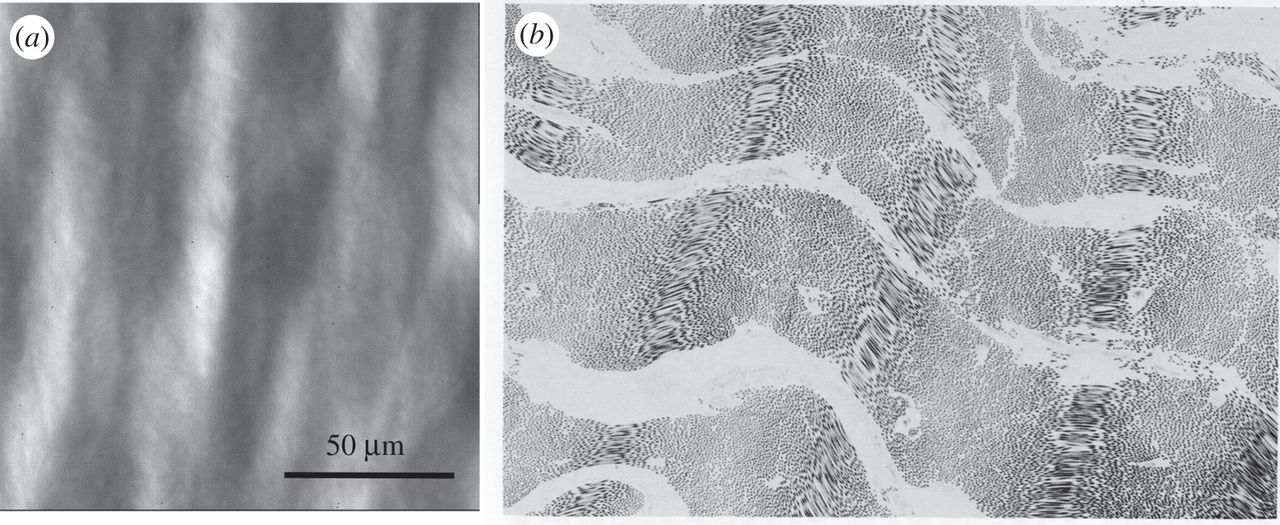
\includegraphics[width=\textwidth]{Images/chapter3/F1large.jpg}
\caption{(a) Photomicrograph of native bovine pericardium showing the undulated collagen fibres (adapted from \cite{sacks_incorporation_2003}). (b) TEM image also of native bovine pericardium clearly showing interrelationships between the undulated collagen fibres and the underlying fibril structures (magnification 4150$\times$; adapted from \cite{nimni_collagen_2018}).}
\label{c3:fig:1}
\end{figure}
%%%%%%%%%%%%%%%%%%%%     end FIGURE     %%%%%%%%%%%%%%%%%%%%

    
    The fiber longitudinal/axial direction is the primary determinant of the stiffness of the tissue composite. Interestingly, collagen fibres typically have a stiffness of 1 GPa \cite{shen_stress_2008,gentleman_mechanical_2003,eppell_nano_2006,yang_mechanical_2008} and extend by no more than 4–5\%. 
    To increase the tissue-level compliance, collagen fibers at the macroscopic scale are sinusoidally crimped \cite{parry_molecular_1988}. Tissue-level stress will not occur until the fiber-level crimp has been straightened. Moreover, the distribution of fiber straightening strains is the mechanism of tissue nonlinearity at large strains \cite{lanir_constitutive_1983,sacks_multiaxial_2003}. Thus, as in many other fields, the connection to the underlying structure can greatly inform our understanding of how collagenous tissues work and guide the development of mathematical models of their mechanical function.


    While there is a wide range of application-specific chemical agents (e.g. riboflavin/UVA cross-linking for corneas), for mechanically-demanding and blood\Hyphdash contacting applications (e.g. BHVs) using collagenous tissues, an aqueous solution of glutaraldehyde (GLUT) is used. GLUT application is necessary to both biochemically and mechanically stabilize the tissue for in vivo use. During the cross-linking process GLUT rapidly permeates the tissue, with the cross-linking process largely complete within an hour and essentially stabilized by 24 hrs. Much of what we know about how GLUT EXLs alter the structures of collagenous tissues was reported by Nimni, Cheung and co-workers \cite{cheung_mechanism_1990,nimni_chemically_1987,cheung_mechanism_1985,gendler_toxic_1984,cheung_presence_1983,cheung_mechanism_1982,cheung_mechanism_1982II}. Briefly, GLUT reacts primarily with e-amino groups of lysyl residues in proteins, with Michael-addition reaction products of Schiff bases usually the final stable products. Based on the spectral characteristics and the molecular weights of the reaction products, it has been predicted that GLUT reacts with free amines to form an intermediate with a molecular weight of about 200 Da. The GLUT–polymer amine complex is self-limiting in size and can undergo internal rearrangement to become chemically inert. An increased molecular length of GLUT polymers from the initial glutaraldehyde and lysyl-residue reaction is more likely than an increased number of cross-linked sites. Following free GLUT depletion by binding to reactive groups, additional GLUT molecules attached to already reacted molecules can give rise to larger GLUT polymers that are able to generate ‘long-range cross-links’ between further removed reactive sites (figure \ref{c3:fig:2}). It is apparent from a mechanical behavior perspective that GLUT-associated chemical cross-linking of the collagen structure and biochemistry can produce complex changes from the native state at the molecular, fibril, fiber and tissue levels.
    
    
%%%%%%%%%%%%%%%%%%%%    begin FIGURE     %%%%%%%%%%%%%%%%%%%%
\begin{figure}
\centering
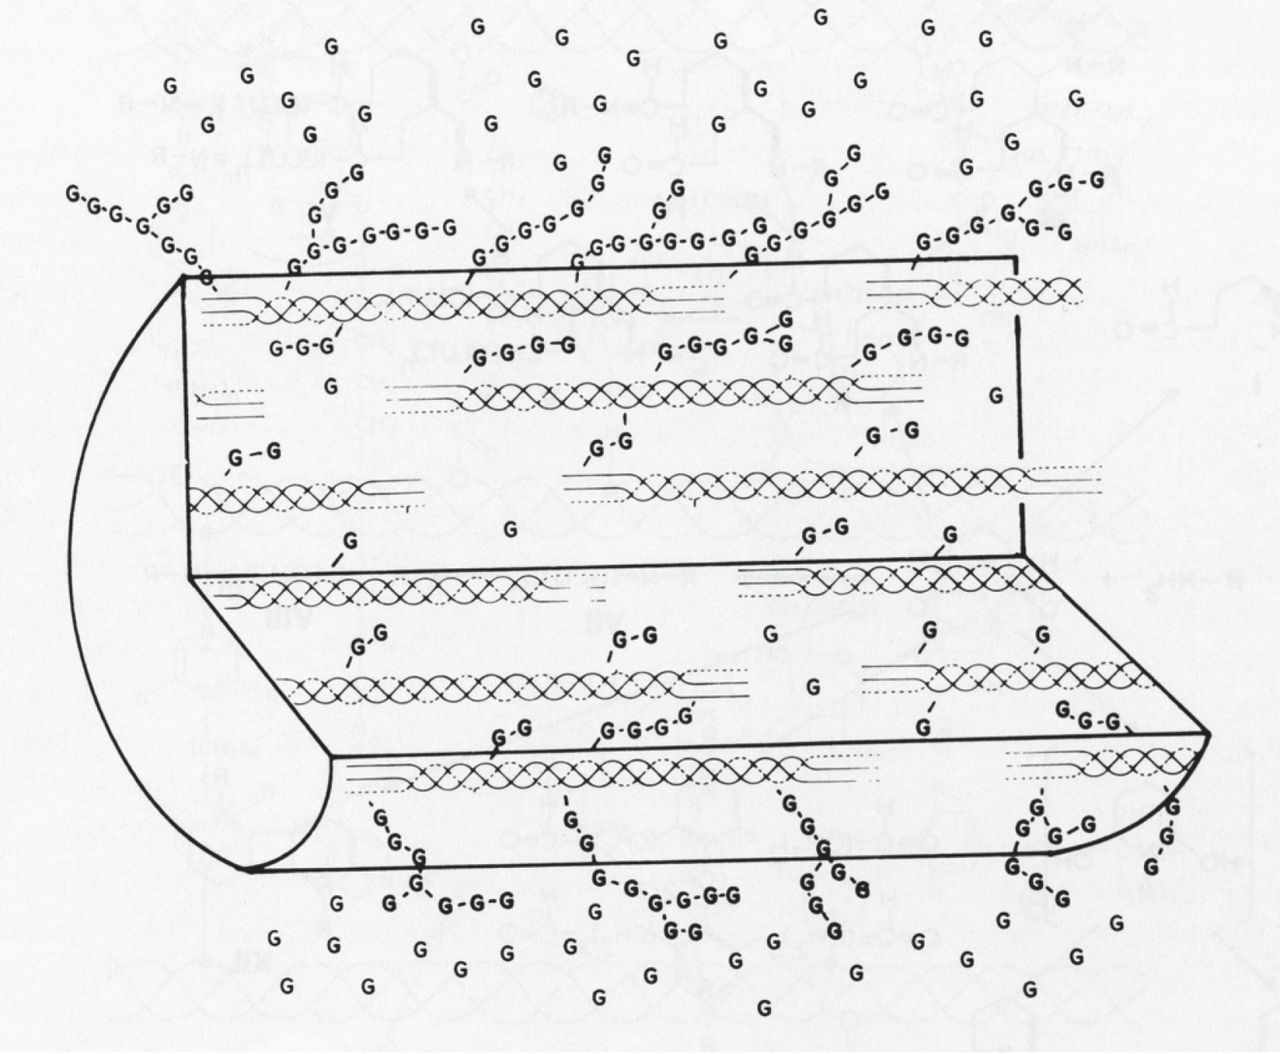
\includegraphics[width=\textwidth]{Images/chapter3/F2large.jpg}
\caption{A diagram showing the interaction of tropocollagen molecules with glutaraldehyde and how cross-links can form. As the concentration of GLUT increases, the number of activation sites and chain length increases, and a limited number of cross-links will form between such molecules (magnification 4150$\times$; adapted from \cite{nimni_collagen_2018}).}
\label{c3:fig:2}
\end{figure}
%%%%%%%%%%%%%%%%%%%%     end FIGURE     %%%%%%%%%%%%%%%%%%%%

    
    To enable improved application of the use of EXL tissues in \textit{in situ} treatment and prosthesis design, the development of physically realistic constitutive models is clearly required. In a previous work, a structural approach was used that incorporated experimentally measured angular distribution of collagen fibers and an assumed isotropic form for the EXL matrix \cite{sacks_structural_2000}. Good agreement with the experimental data was observed, supporting the basic approach. An important utility of that early model was its ability to separate the effects of the fibers and matrix. However, it was only a first step; other factors such as bending rigidity of EXL fibers, fiber-fiber interactions, and fiber-matrix interactions were not considered. Moreover, the experimental data were reduced under the assumption of an isotropic Fung model; no rigorous investigation of the most appropriate form was undertaken.
    
    
    The focus of the present work is to more fully investigate the underlying characteristics of the effects of EXLs on soft collagenous tissues and to use this information to develop a meso-scale (i.e. at the level of the fiber) structural constitutive model. In particular, we explored the following questions of the effects of EXLs on native collagenous tissues: (i) what are the effects on individual collagen fibres, (ii) what are the effects on single collagen fibre ensembles, (iii) are there interactions between fibre ensembles, and (iv) what is the functional form of the effective matrix response? This was done by exploiting experimental data from \cite{sun_biaxial_2003}, wherein structurally controlled pericardial specimens were tested in the native state and then the EXL state. From these results, a comprehensive structural constitutive model was developed for EXL collagenous tissues and its predictive capability was evaluated. We note that, while we ultimately seek the micro-mechanical basis for macro-scale function, the present work is focused on a fiber-ensemble level approach.
    
    
    

